\documentclass[parskip,10pt,abstracton]{scrartcl}
\usepackage[top=3cm, bottom=3cm, left=3cm, right=3cm]{geometry}
\usepackage{polyglossia}
\setmainlanguage{german}
\pagenumbering{gobble}

\usepackage{setspace}
\onehalfspacing

% ------------------------------------------------------------------------------------
% packages
\usepackage{graphicx}
\usepackage{tikz}
\usetikzlibrary{arrows,shapes,positioning, shadows,trees}
\usepackage{enumerate}

% ------------------------------------------------------------------------------------
% Header
% ------------------------------------------------------------------------------------
\renewcommand*{\maketitle}{%
	{\centering\LARGE\sffamily\bfseries Aufgabe 4: Der Papierprototyp \par}
	\vspace{3em}
}

% ====================================================================================
% Document
% ====================================================================================
\begin{document}

\maketitle

% ------------------------------------------------------------------------------------

% AUFGABE
  % Prototyp mittels Fotos und Erklärungen dokumentieren:
  % Grundaufbau
  % Funktionalitäten
  % 3 Szenarien durchgehen

% ------------------------------------------------------------------------------------
\section*{Grundaufbau}

Startseite:
\begin{center}
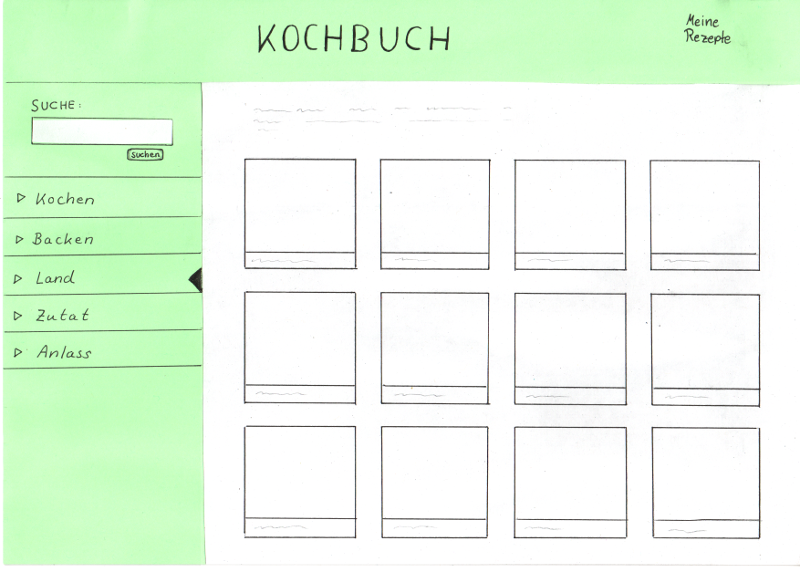
\includegraphics[scale=0.4]{Prototyp/home.png}
\end{center}

Die Startseite enthält einen kurzen Begrüßungstext mit einer kurzen Erklärung der Navigation und Bilder von verschiedenen Rezepten.\\
Rechts oben befindet sich der Menüpunkt der zum persönlichen Kochbuch, beziehungsweise zum Login führt.\\
Auf der rechten Seite ist eine einklappbare Möglichkeit, die Rezepte nach Belieben zu filtern. Entweder nach Suchbegriffen oder nach verschiedenen Kategorien, die auf dem Prototypen in einer Auswahl dargestellt sind.

Rezeptseite:
\begin{center}
\includegraphics[scale=0.4]{Prototyp/plätzchenrezeptseite.png}
\end{center}

Eine Rezeptseite enthält Bild, Zutaten, Zubereitung und Kommentare zu einem Rezept. In dem Bereich auf der rechten Seite befindet sich der Button um das Rezept zu speichern. Ist man nicht eingeloggt, wird dazu zuerst aufgefordert, wenn der Button betätigt wird.
Außerdem sind dort Informationen zum Aufwand des Rezepts, den Kategorien, denen es zugeordnet ist und Ähnliches.

% ------------------------------------------------------------------------------------
\section*{Funktionalität der Navigation}

Einklappen der Seitennavigation:
\begin{center}
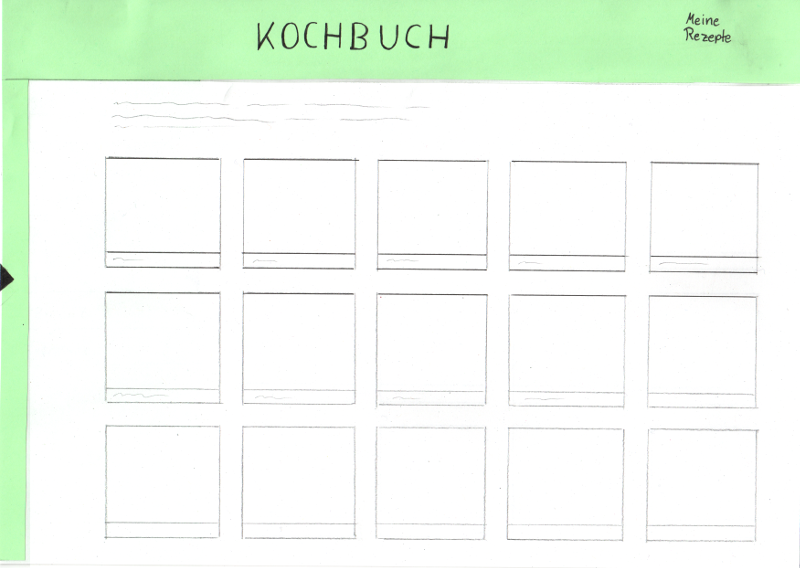
\includegraphics[scale=0.4]{Prototyp/home_menuhidden.png}
\end{center}

Die Seitennavigation kann einfach ein- und ausgeklappt werden.

horizontales Menü: meine Rezepte
\begin{center}
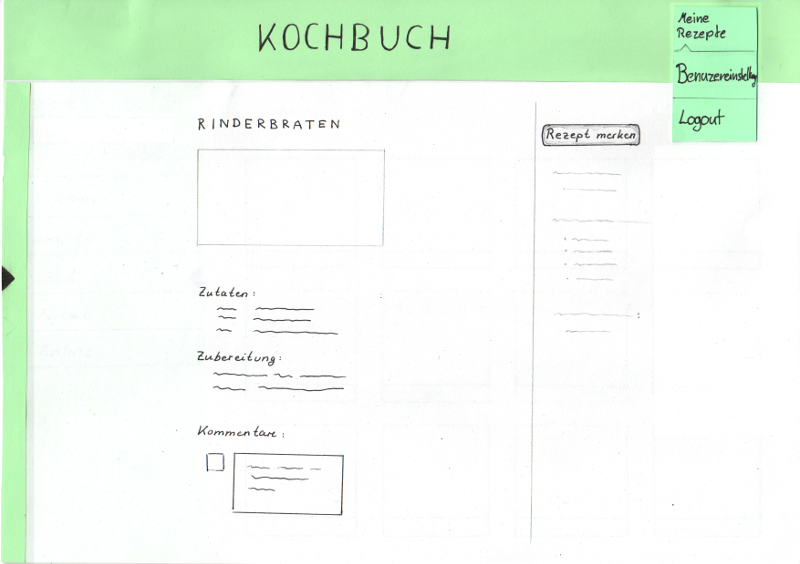
\includegraphics[scale=0.4]{Prototyp/menu_eigeneRezepte_menuhidden.png}
\end{center}


Die einzelnen Menüpunkte sind aufklappbar:

Menü: Kochen
\begin{center}
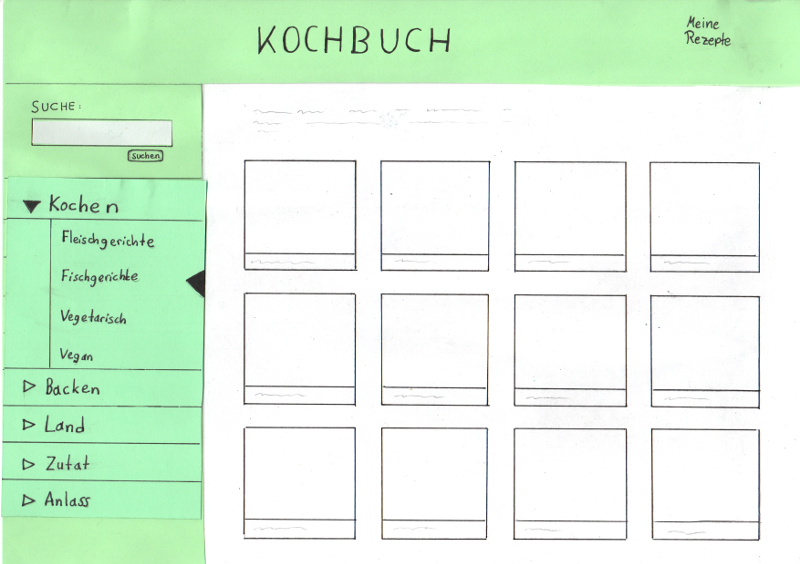
\includegraphics[scale=0.4]{Prototyp/menu_kochen.png}
\end{center}

Menü: Backen
\begin{center}
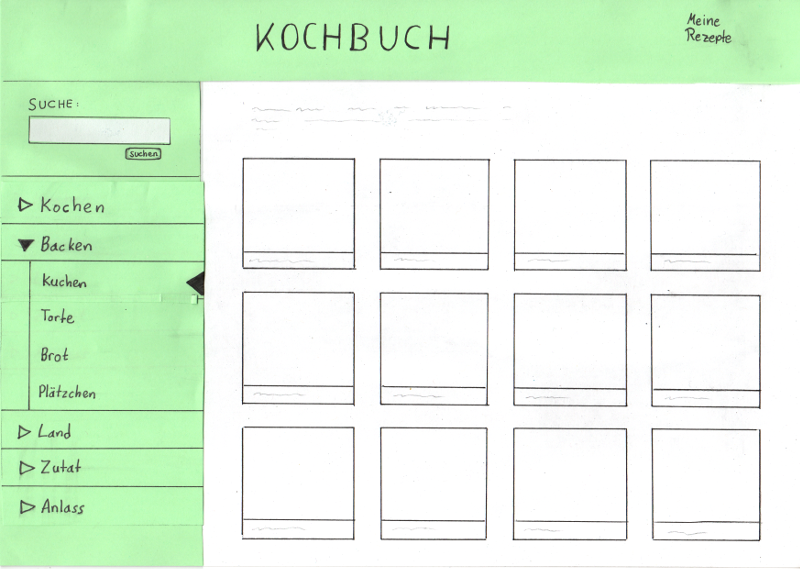
\includegraphics[scale=0.4]{Prototyp/menu_backen.png}
\end{center}

Menü: Zutat
\begin{center}
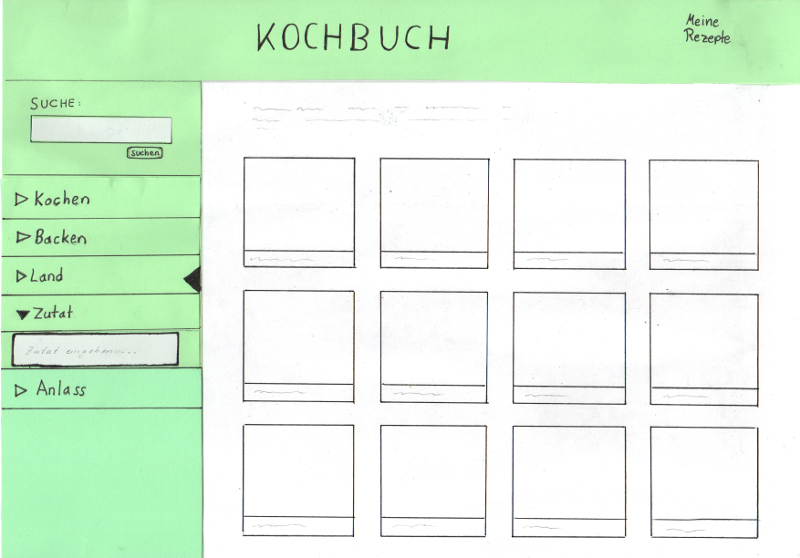
\includegraphics[scale=0.4]{Prototyp/menu_zutat.png}
\end{center}


\pagebreak
% ------------------------------------------------------------------------------------
\section*{Die 3 Szenarien}

\subsection*{Szenario 1: Max will Plätzchen backen}

Er verwendet die Suchfunktion, gibt "Plätzchen" ein und erhält Plätzchenrezepte.
\begin{center}
\includegraphics[scale=0.4]{Prototyp/plätzchensuche.png}
\end{center}

Er wählt eines aus und wird auf die entsprechende Rezeptseite gebracht.
\begin{center}
\includegraphics[scale=0.4]{Prototyp/plätzchenrezeptseite.png}
\end{center}


\subsection*{Szenario 2: Karl hat nur bestimmte Zutaten da}

Er wählt im Seitenmenü "Zutat" aus...
\begin{center}
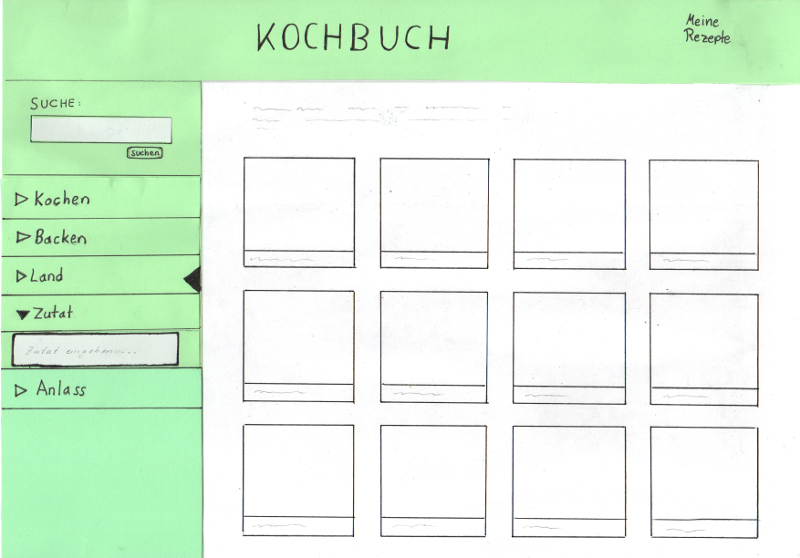
\includegraphics[scale=0.4]{Prototyp/menu_zutat.png}
\end{center}

... und gibt die Zutaten ein, die ihm zur Verfügung stehen: Nudeln, Hackfleisch und Tomaten
\begin{center}
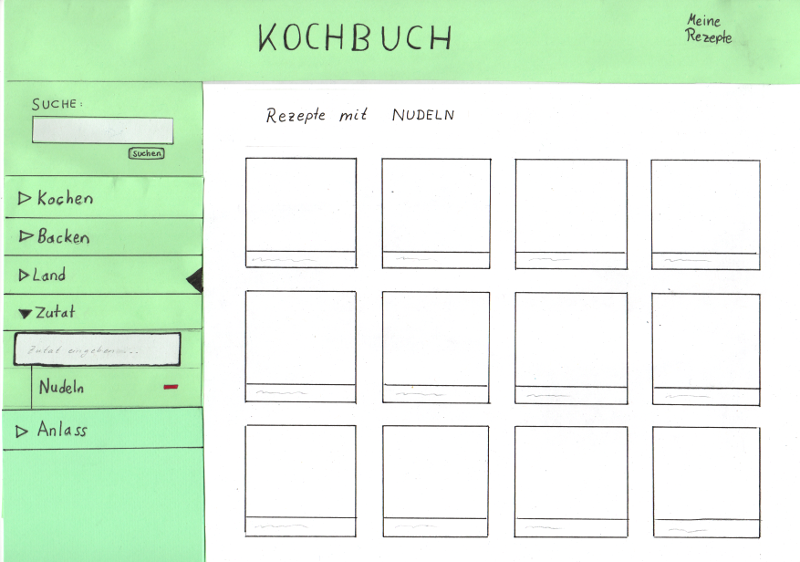
\includegraphics[scale=0.4]{Prototyp/menu_zutat_nudeln.png}\\[1em]
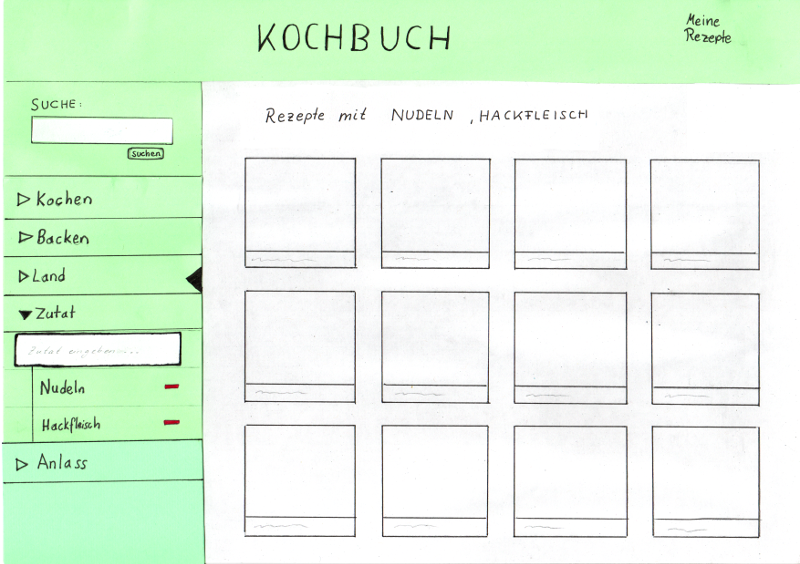
\includegraphics[scale=0.4]{Prototyp/menu_zutat_nudelnhackfleisch.png}\\[1em]
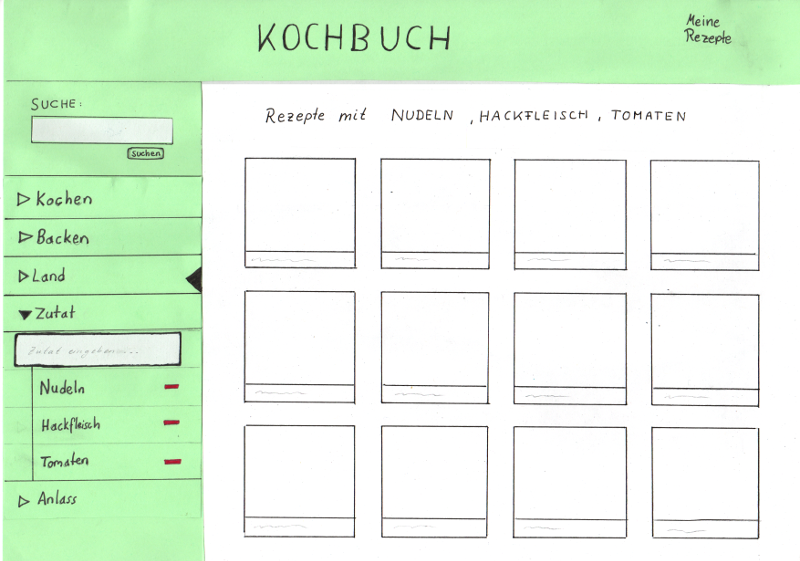
\includegraphics[scale=0.4]{Prototyp/menu_zutat_nudelnhackfleischtomate.png}
\end{center}


\subsection*{Szenario 3: Anna lässt sich inspirieren}

Anna klappt das Seitenmenü ein, um auf der gesamten Breite die Bilder der Rezepte betrachten zu können.
\begin{center}
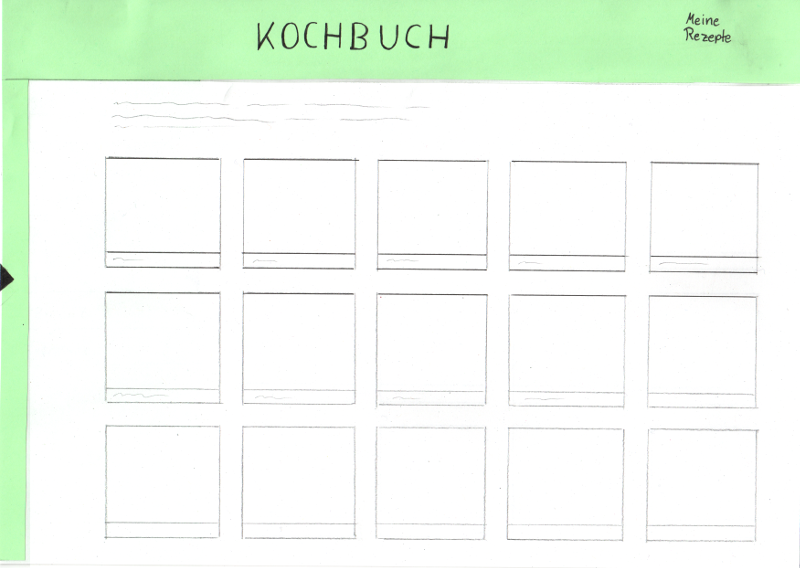
\includegraphics[scale=0.4]{Prototyp/home_menuhidden.png}
\end{center}

Sie scrollt durch die Bilder und sieht sich ein bestimmtes Rezept an.
\begin{center}
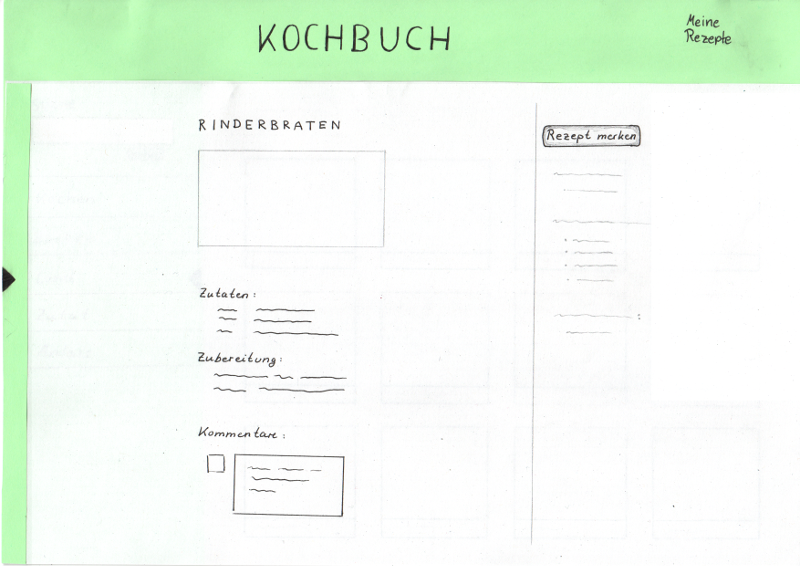
\includegraphics[scale=0.4]{Prototyp/rezeptseite_menuhidden.png}
\end{center}

Sie klickt auf "Rezept merken" und sieht sich dann unter "meine Rezepte" ihre bisher gespeicherten Rezepte an.
\begin{center}
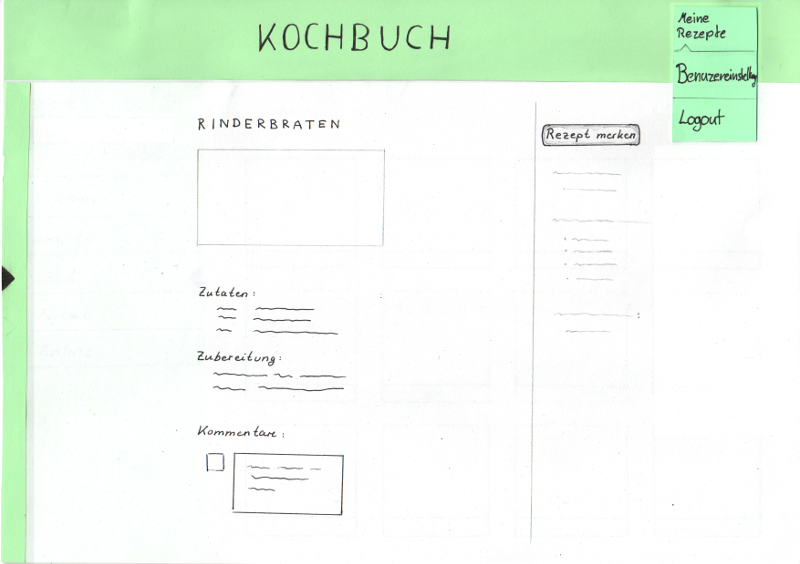
\includegraphics[scale=0.4]{Prototyp/menu_eigeneRezepte_menuhidden.png}\\[1em]
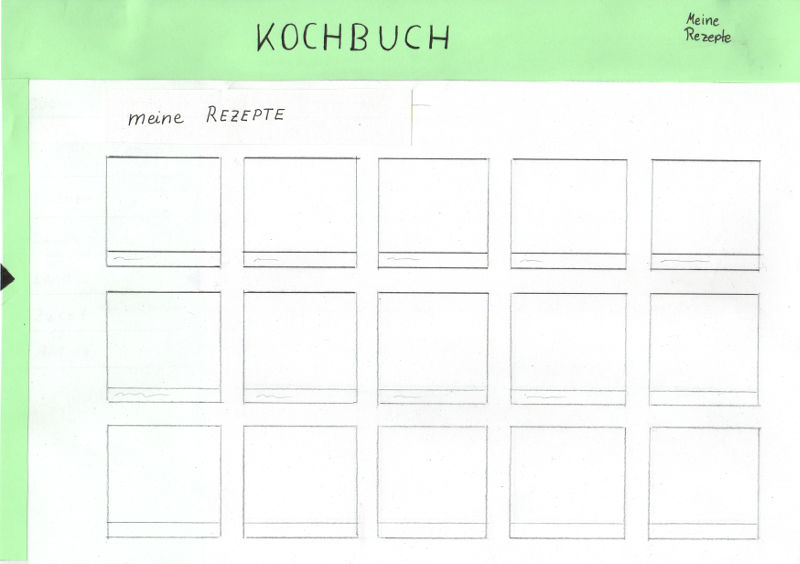
\includegraphics[scale=0.4]{Prototyp/meineRezepte_menuhidden.png}
\end{center}

\end{document}



